\documentclass[twoside,11pt,ShortChapTitles]{BYUTextbook}

\usepackage{soul}
\renewcommand{\vec}[1]{\ensuremath{\mathbf{#1}}}
\usepackage{siunitx}
\sisetup{round-mode = figures,
  round-precision = 3, scientific-notation=true}
  \usepackage{marginfix}

\usepackage{mathtools}
\renewcommand{\chaptername}{Lab}

\setcounter{chapter}{8}

\begin{document}
\chapter{Measurement and Uncertainty III}

We should tie our numerical modeling knowledge into our understanding of
uncertainty. We want to be able to numerically predict the outcome of an
experiment. But that prediction should come with an uncertainty. How can we
find an uncertainty for something we found numerically?

Let's think about what we have been calling the high/low method of finding
an uncertainty. Each measurement we make has an uncertainty. If we use those
measurements to calculate things like we did a few weeks ago to find the
value of $g,$ we have to combine or \emph{propagate} the uncertainties. We
used large equations with derivatives to do this when we knew the function
that described our prediction. But now we don't have an equation that tells
us how a ball will fall with air resistance. We need another method for
finding the uncertainty in a numerical solution like our Euler method. But
we can use our high/low method to develop a new, computational method of
finding the error.

Think back to our lab where we measured $g.$ One way to find the uncertainty
was to use our equation to find the combination of values that gave the
largest estimate for $g.$ Then find the combination of values that gave the
smallest estimate for $g.$ For example, when you found $g$ using the
pendulum your equation should have been something like
\[
g=4\pi ^{2}\frac{L}{T^{2}}
\]%
we can find the uncertainty by taking
\[
g_{\max }=4\pi ^{2}\frac{L_{\max }}{T_{\min }^{2}}
\]%
where $L_{\max }=L+\delta L$ and $T_{\min }=T-\delta T.$ We can also find
\[
g_{\min }=4\pi ^{2}\frac{L_{\min }}{T_{\max }^{2}}
\]%
And then an estimate for the uncertainty would be half the difference
between $g_{\max }$ and $g_{\min .}$

Of course we can't exactly do this for our ball case because we don't know
the function for our ball fall with air resistance. We don't know whether to
use max or min input vales (like $L_{\max }$ and $T_{\min }$ above).
Combinations that make the maximum distance and the minimum distance do
exist. We just don't know how to form them. We have lots of inputs to our
Euler's method. Each has uncertainty. How do we know which ones to use as
maximum values and which ones to use as minimum values? We know that things
get funny when we divide, so without knowing the actual function we don't
know how to combine the input values to get the maximum or minimum distance.

The answer is that we will have to guess, but guess systematically. That may
sound unsettling, but we have a computer that can help us to guess. We can
choose random values for each of our inputs such that the value we choose is
within the uncertainty for each measurement. Then run the code and see how
far away the ball gets when it lands. Then choose a new random set of inputs
and see if it get's farther. The computer can do this quickly, so we can run
hundreds of combinations in just a few minutes. For our
ball-shot-out-of-a-cannon model, say, we used

\begin{itemize}
\item {\small The initial }$y${\small \ position of the projectile }$%
y=\left( 27.00+1\right) \text{cm}$

\item {\small The initial speed of the projectile. }$\left( 6.8+0.2\right)
\text{m}/\text{s}$

\item {\small The launch angle for the projectile (measured from the
positive }$x${\small \ axis) }$\left( 45+1\right)^\circ$

\item {\small The mass of the projectile.}$\left( 0.0003+0.00001\right)
\text{kg}$

\item {\small The radius of the projectile.}$\left( 0.0125+0.000\right) 1%
\text{m}$

\item {\small The drag coefficient for the projectile }$0.46+0.2$

\item {\small The density of the air the projectile travels through }$\left(
1.23+0.1\right) \text{kg}/\text{m}^{3}$

\item {\small the acceleration due to gravity is }$\left(
9.8004+0.001\right) \text{m}/\text{s}$
\end{itemize}

Then we could try again with the choices

\begin{itemize}
\item {\small The initial }$y${\small \ position of the projectile }$%
y=\left( 27.00-1\right) \text{cm}$

\item {\small The initial speed of the projectile. }$\left( 6.8-0.2\right)
\text{m}/\text{s}$

\item {\small The launch angle for the projectile (measured from the
positive }$x${\small \ axis) }$\left( 45-1\right)^\circ$

\item {\small The mass of the projectile.}$\left( 0.0003-0.00001\right)
\text{kg}$

\item {\small The radius of the projectile.}$\left( 0.0125-0.000\right) 1%
\text{m}$

\item {\small The drag coefficient for the projectile }$0.46-0.2$

\item {\small The density of the air the projectile travels through }$\left(
1.23-0.1\right) \text{kg}/\text{m}^{3}$

\item {\small the acceleration due to gravity is }$\left(
9.8004-0.001\right) \text{m}/\text{s}$
\end{itemize}

If we do this hundreds of times, each time with a different combination
input parameters, we can take a mean and standard deviation and have our
predicted value and uncertainty for our distance that the ball will go.

We might not get the actual maximum (or minimum distance) combination
without trying millions of combinations (maybe more!). But knowing some
statistics, we can still estimate the uncertainty We can average our
predicted distances and use this average as our prediction for where the
ball will hit. We can take a standard deviation of our predicted distances
and use this for an uncertainty. A standard deviation of the mean might be
even better.

This is a little like throwing darts at a target and taking the mean and
standard deviation to tell where we were aiming and with what precision. But
now we are doing that with our numerical prediction. We make many
predictions with our inputs within their respective uncertainties, and then
average at the end.

We know that when we use a standard deviation for our uncertainty, we miss
some cases, only 68\% of the predicted distances will fall within that
standard deviation. So it is not as important to run our code millions of
times if we can make due with a standard deviation as our estimate of
uncertainty. A few hundred combinations should be enough.\pagebreak

\section{Assignment: Modeling and Uncertainty}

In this lab we will finally test our numerical modeling of a projectile. We
will use our spring cannons and shoot balls that have large drag
coefficients. \textbf{Be careful not to shoot people, including you--don't
look down the barrel of the cannon! Also, don't load the cannon by pushing
down on the ball in the cannon, set the spring first and then gently put in
the ball If you push on the Styrofoam balls you will have flat balls that
don't match our models. }

There is too much to do in this lab to have everyone do all the parts. You
will have to split up your group. So how do you record all the experiment if
you only do part of it? The way this is done is to write down the results
obtained by the other subgroups, and refer to their lab notebooks for the
details.

\begin{enumerate}
\item \textbf{Predict} the maximum range for the path of a Styrofoam ball
(or a plastic ball if we don't have any Styrofoam balls) shot out of the
spring cannon. Do this with a numerical model of the ball's flight path
written by one (or more) of the members of your group that has been changed
so that it can find the error estimate as described in today's lab reading.

\item Determine the uncertainty in your prediction with your new code that
chooses values for the input parameters randomly from within the parameter
uncertainty ranges. This\sidenote{Randomly choosing values lets the Central Limit Theorem apply.} is actually more efficient than trying to pick
values in a non-random way to cover all possible combinations of
uncertainties! You will need to take about $100$ or more sets of parameters
to get a good estimate, but if you built your code so you can easily change
your parameters, this will go quickly (if you put actual numbers into your
equations in the previous labs, it might be faster to fix your Python code
first to make this part go more quickly. If you need help, call me over).


\begin{itemize}
\item This function will help you randomly generate values in your uncertainty range.  Some parts were intentionally left blank for you to fill in.
\begin{Verbatim}
#Import a random number generator
from random import random

#Create a function that takes in a value and an uncertainty
#and returns a value in that range
def select_val(val,uncert):
    #Generate a random number between 0 and 1
    my_rand = random()
    #Shift the random number so that it falls between -1 and 1
    my_rand =
    #Convert that random number to a shift away from the value
    val_shift =
    #Give back the shifted value
    return val+val_shift

\end{Verbatim}



\item You want to do this for every variable that has
uncertainty, and you want to do the calculation many times so you get a good
idea of the precision of your answer. Here is a figure showing an example
result:

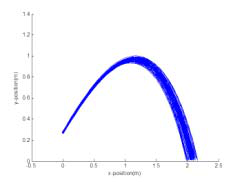
\includegraphics[scale=0.6]{Lab9_figs/old_images-058.png}

\item Additionally, you need to be able to find where the ball hits the ground.  You can do this by either changing your Euler \code{for} loop into a \code{while} loop, or by inserting an \code{if}\sidenote{The command \code{break} will tell your program to exit whatever loop it is currently in.} statement.

\end{itemize}
\item You will need to find the drag coefficient. A subteam should find a
value (and uncertainty) for the drag coefficient. One way to do this is to
use our high speed cameras and film the ball dropping. Since there is
significant air resistance, the ball will reach terminal speed. At this
point, there is no acceleration, so
\begin{eqnarray*}
\sum F &=&0=R-F_{g} \\
F_{g} &=&R \\
mg &=&\frac{1}{2}D\rho Av^{2}
\end{eqnarray*}%
so%
\[
D=\frac{2mg}{\rho Av^{2}}
\]%
Since we know or can measure everything except $D,$ we can solve for $D.$
Use $g=\left( 9.8004\pm 0.0001\right) \text{m}/\text{s}$ and $\rho =\left(
1.23\pm 0.1\right) \text{kg}/\text{m}^{3}.$

\begin{itemize}
\item The rest of the values you will need to measure. Use the digital
camera and Logger Pro to estimate the terminal velocity. You will have to
drop the ball from high up to get a good value (you have to give it time to
reach terminal velocity). Near the ground there can be problems due to the
air flow hitting the ground, so don't use positions that are close to the
ground.

\item I suggest you have a team of people from your group do this while a
second team modify your MatLab code. Remember you need an uncertainty in $D.$
\end{itemize}

\item Verify the prediction. Did the ball land within your error range? If
you use the digital cameras again for this part, you can determine if the
flight path falls within the range of possible flight paths. A figure like
the following might help you decide:

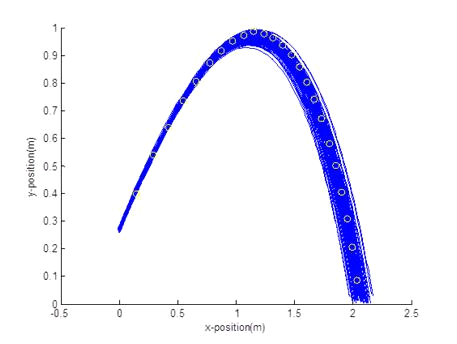
\includegraphics[scale=0.5]{Lab9_figs/old_images-059.png}

\item Does the data support your modeling prediction? If not, what is likely
the problem?

\begin{itemize}
\item In your discussion make sure your other team members understand the
part of the project that you did.

\item You might consider having a third team collect data for the ball shot
with the digital camera while the first two teams are working on the drag
coefficient and the numerical prediction.
\end{itemize}


\end{enumerate}

\end{document}
